\section{The EXAFS Equation}

\begin{frame}
  \frametitle{The EXAFS Equation}  % XAFS Analysis with {\feff}}

\begin{cenpage}{110mm}

  The XAFS Equation used with {\feff}:

  \[
  \chi(k) = \sum_j {{ S_0^2 {\Blue{N_j}} {\Red{f_j(k)}}  e^{-2R_j/{\Red{\lambda(k)}}}
      e^{-2k^2{\Blue{\sigma_j^2}}}}\over{k{\Blue{R_j}}^2}}
  {\sin[{2k{\Blue{R_j}} + {\Red{\delta_j(k)}}} ]}
   \]

\begin{itemize}
  \item $\Red{f(k)}$ and $\Red{\delta(k)}$ are  {\emph{photo-electron scattering
        amplitude and phase}}:
    \begin{itemize}
    \item Energy dependent    \hspace{3mm}  $k \sim \sqrt{(E-E_0)} $.
    \item Depend on $Z$ of the scattering atom(s).
    \item Non-trivial: must be calculated or carefully extracted from  measured spectra.
    \end{itemize}

\item $\Red{\lambda(k)}$ tells how far the photo-electron can travel.

\item The sum is over {\RedEmph{Scattering Paths}} of the photo-electron,
  from absorbing atom to neighboring atom(s) and back.  May include
  {\BlueEmph{multiple scattering}}!

\end{itemize}

   \onslide+<2->

   \begin{postitbox}{64mm}
     If we know $\Red{f(k)}$,  $\Red{\delta(k)}$, and $\Red{\lambda(k)}$, we can get:
     \begin{itemize}
     \item ${\Blue{R}}$ --  near neighbor distance.
     \item ${\Blue{N}}$ -- coordination number.
     \item ${\Blue{\sigma^2}}$ -- mean-square  disorder in ${\Blue{R}}$.
     \end{itemize}
   \end{postitbox}

\end{cenpage}
\end{frame}




\section{{\feff}}


\subsection{Scattering Amplitude and Phase}
\begin{frame} \frametitle{Scattering Amplitude and Phase-Shift:
    ${f(k)}$ and ${\delta(k)}$ }

  The scattering amplitude ${\Red{f(k)}}$ and phase-shift
  ${{\Red{\delta(k)}}}$ depend on Z:

    \vmm

    \begin{tabular}{ll}
      \begin{minipage}{55mm}
        \rgraph{55mm}{scatt_amp}
        \end{minipage} &
        \begin{minipage}{55mm}
          \rgraph{55mm}{scatt_pha}
      \end{minipage}\\

      \begin{minipage}{55mm}
      $\Red{f(k)}$ peaks at higher  $k$ as Z increases.  Heavy
        elements, have a characteristic dip in $\Red{f(k)}$, and
        scatter to high $k$.  

        {\bf{Note: O is done at $k>15\rm\AA^{-1}$}}


      \end{minipage}
      &
      \begin{minipage}{55mm}

        The phase shift $\Red{\delta(k)}$ also shows strong Z
        dependence, and has sharp jumps for heavy elements where $f(k)$ dips.

        {\bf{Note:  $\delta(k) \approx -k$! }}
      \end{minipage} \\
    \end{tabular}

\begin{postitbox}{50mm}
  Z can usually be determined to $\pm 5$.

\vmm
  Fe and O can be distinguished.

\vmm
  N  and O cannot be distinguished.
\end{postitbox}
\vfill
\end{frame}


\begin{frame} \frametitle{ $\lambda(k)$: The Photo-Electron Mean-Free Path }

 \begin{cenpage}{102mm}
  The $ e^{-2R/\lambda(k)} $ term in the XAFS Equation accounts for how far the
   photo-electron can travel and still return (in phase) to the excited atom.
 \begin{columns}
   \begin{column}{55mm}
     \rgraph{57mm}{lambda}
   \end{column}
   \begin{column}{60mm}

     This includes both:

     \begin{itemize}
     \item  inelastic scattering of photo-electron.
     \item  finite lifetime of the core-hole (fs).
     \end{itemize}
     \vmm

   \end{column}
 \end{columns}

 \vmm\hrule\vmm

The photo-electron goes only {10 to 20 \AA}  over most of the EXAFS region. 

 \begin{postitbox}{80mm}
     The $\lambda$ and $1/R^{2}$ terms make EXAFS a  {\RedEmph{local probe}}.
   \end{postitbox}

  \end{cenpage}
\end{frame}



\begin{frame}  \frametitle{EXAFS Analysis Strategy:  How to get $N$, $R$, etc?}

  \begin{cenpage}{99mm}

    % \begin{center}\begin{minipage}[t][12mm]{90mm}
      \[
      \chi(k) = \sum_j {{ S_0^2 {\Blue{N_j}} {\Red{f_j(k)}}  e^{-2R_j/\lambda(k)}
          e^{-2k^2{\Blue{\sigma_j^2}}}}\over{k{\Blue{R_j}}^2}}
      {\sin[{2k{\Blue{R_j}} + {\Red{\delta_j(k)}}} ]}
      \]
   %% \end{minipage}  \end{center}

   \vmm
   Steps:
   \begin{enumerate}
   \item Calculate theoretical XAFS spectra  with {\feff},  starting with a guess of the local structure.
   \item  {\RedEmph{Refine}} $R$, $N$, and $\sigma^2$  to best match  experimental data.
   \item Compare lots of refined models.
   \end{enumerate}

\vmm \vmm \hrule \vmm\vmm

 Questions you might have (and we might answer!):

  \begin{itemize}
  \item How do we run {\feff} to generate $\Red{f(k)}$, $\Red{\delta(k)}$,
    and  $\Red{\lambda(k)}$?
  \item What correction factors do we need to worry about?
  \item How do we fit experimental data?
  \item How do we interpret the results?
  \item Any advice for making all this, um, easier?
  \end{itemize}

\vfill
   \end{cenpage}

\end{frame}



\subsection{{\feff}}
\begin{frame}
  \frametitle{{\feff} Calculation Overview: What does {\feff} do? }

  \begin{cenpage}{112mm}
  {\feff} calculates the EXAFS {$\chi(k)$}  by simulating the scattering of a
  photo-electron along all scattering paths from a selected absorbing atom within
  a  cluster of atoms.
  \end{cenpage}

    \vmm

  \begin{enumerate}
    \onslide+<1->\item   build atomic potentials.   To  simplify calculations,
      \begin{center}
        \begin{tabular}{ll}
          \begin{minipage}{75mm}
            Use the {\BlueEmph{Cup-Cake Tin Approximation}}:
            atomic potentials up to a uniform Fermi level -no chemical bonding.

            \hspace{2mm}(Some people call this ``Muffin-Tin'' Approximation)
          \end{minipage}
          &
          \begin{minipage}{30mm}
            \vspace{1mm} 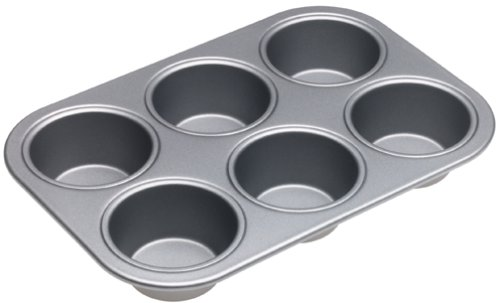
\includegraphics[width=27mm]{figs/theory/muffintin2}
          \end{minipage}
        \\
      \end{tabular}
    \end{center}


  \onslide+<2->\item determine important scattering paths.

    \begin{itemize}
    \item Build paths from a selected {\BlueEmph{central atom}} in a cluster of atoms
    \item decide which ones are ``degenerate'' (=``'equivalent'',   !=``degraded state'')
    \item decide which ones are unimportant for XAFS
    \end{itemize}


  \onslide+<3->\item move photo-electron along path to determine
    $\Red{f}$ and $\Red{\delta}$ as a function of $k$:

    \begin{center}
      propagate $\Rightarrow$ scatter $\Rightarrow$ propagate $\Rightarrow$ \ldots.
    \end{center}

  \end{enumerate}

\end{frame}

\subsection{{\feff}   complications}
\begin{frame} \frametitle{{\feff}: what's so hard about that??}

  \begin{cenpage}{105mm}
    {\feff} includes sophisticated techniques to calculate of \feffc{f(k)},
    \feffc{\delta(k)}, and \feffc{\lambda(k)}.

    \begin{description}
    \item[\RedEmph{Curved Wave Effects}] the photo-electron goes out as
      spherical wave and scatters from atoms with finite size.

    \item[\RedEmph{Muffin-Tin Approximation:}] Makes the calculations
      tractable, but is an approximation.

    \item[\RedEmph{Multiple Scattering}]  the photo-electron can scatter
      multiple times. Most important at low $k$ and for \BlueEmph{linear paths}.

    \item[\RedEmph{Extrinsic Losses}] {\feffc{\lambda(k)}}: self-energy and
      core-hole lifetime.

    \item[\RedEmph{Intrinsic Losses}] {\feffc{S_0^2}}: the absorbing atom
      relaxes to the presence of the hole left in the core electron level.

    \item[\RedEmph{Polarization Effects}] synchrotron beams are highly
      polarized, which needs to be taken into account.  This is simple for
      $K$ edges ($s\rightarrow p$ is dipole), but slightly more complicated for
      $L$ and $M$ edges.

    \end{description}

    \end{cenpage}
\vmm
\begin{center} Usually, you don't have to worry about these things.\end{center}

\end{frame}


\section{{\feff} complications}

\subsection{{\feff} complication \#1: Multiple Scattering}
\begin{frame} \frametitle{{\feff} complication \#1: Multiple Scattering}

  \vmm
\begin{columns}
  \begin{column}{50mm}
  The photo-electron can scatter multiple times before getting back to the
  absorbing atom:

  \begin{center}
    \rgraph{50mm}{mspaths}
  \end{center}

  \end{column}
  \begin{column}{60mm}

  A {\Blue{Path Formalism}} is used in the  calculation:

  \begin{center}
    propagate $\Rightarrow$ scatter $\Rightarrow$ propagate $\Rightarrow$ \ldots.
  \end{center}

  \vmm  
  \vmm {\Red{Single Scattering}}  usually important.

  \vmm {\Red{Triangle Paths}} with angles $ 45 < \theta <
  135^{\circ}$ scatter weakly, but there are lots of them.

  \vmm {\Red{Linear paths}} with angles $\theta \approx 180^{\circ}$
   are very strong: the photo-electron is {\Red{focused}} through an atom.
   Can be used to measure bond angles\ldots

  \end{column}
  \end{columns}

   \begin{postitbox}{92mm}
     \Red{ A {\feff} Path looks the same for Single and Multiple
       Scattering}
   \end{postitbox}
\end{frame}

\subsection{{\feff} Complication \#2: S02}
\begin{frame} \frametitle{{\feff} complication \#2: $S_0^2$, the  Amplitude Reduction Term}

  \vmm
    \begin{cenpage}{110mm}

  The {\RedEmph{other}} electrons in the absorbing atom can relax due to
  the core-hole, giving an {\Red{Amplitude Reduction Term}}:

   \vmm
   \[
   S_0^2 =  {  |{\langle \Phi^{N-1}_f |\Phi^{N-1}_0 \rangle}|^2}
   \]

    \vspace{1mm}

    ${| \Phi^{N-1}_0 \rangle }$ = $(N-1)$ electrons in unexcited atom.

    ${\langle \Phi^{N-1}_f|}$   = $(N-1)$ electrons, relaxed by core-hole.

    \vmm

    \onslide+<2->
    ${S_0^2}$ is taken as a constant: \hspace{3mm}  $ 0.7 < S_0^2 < 1.0 $.

    and may be used as a Fitting Parameter that multiplies {$\chi$}:

    \vmm \vmm
    \begin{center}
      {\Red{ ${S_0^2}$ is Completely Correlated with $N$      (!!!)}}
    \end{center}


    \begin{postitbox}{68mm}
      $S_0^2$ is usually constant for  data measured on
      the same edge {\bf{and}} beamline (energy resolution).
    \end{postitbox}

    Most Common Approach: Determine $S_0^2$ from experimental data on a
    system with known $N$, and then use that for unknown data. 

    \vmm

    \end{cenpage}

\end{frame}
